% !TEX root = Projektdokumentation.tex

\newglossaryentry{XML External Entitiy} {name={XML External Entitiy-Attacke},description={Eine Attacke, welche gegen einen XML-Input-Parser geht. Sie tritt auf, wenn der XML-Input einen Verweis auf eine externe Server-Ressource enthält, auf welche der Angreifer gar keinen Zugriff haben dürfte, und der Parser dies nicht prüft. \cite{xxe}}}

\newglossaryentry{Refactoring}{name={Refactoring},
	description={Refactoring bezeichnet die manuelle oder automatisierte Strukturverbesserung von Quelltexten unter Beibehaltung des beobachtbaren Programmverhaltens. Dabei sollen die Lesbarkeit, Verständlichkeit, Wartbarkeit und Erweiterbarkeit verbessert werden, mit dem Ziel, den jeweiligen Aufwand für Fehleranalyse und funktionale Erweiterungen deutlich zu senken. \cite{_refactoring_2016}}
}

\newglossaryentry{URL}{name={URL},description={\begin{quote}
			Uniform Resource Locator (URL) ist eine Adressierungsform für Internetadressen, die vor allem innerhalb des World Wide Web (WWW) zur Anwendung kommt.
		\end{quote} \cite{url}}}

\newglossaryentry{Denial of Service}{name={Denial of Service},description={\begin{quote}
			\glqq Durch einen Denial-of-Service (DoS)-Angriff werden Dienste in ihrer Funktionalität beeinträchtigt und stehen Nutzern sowie Unternehmen nur eingeschränkt zur Verfügung.\grqq
		\end{quote} \cite{dos}}}

\newacronym{AJAX}{AJAX}{Asynchronous Javascript And XML}



\section{Verbesserung der bestehenden Lösung}

\subsection{\gls{Refactoring} und Fehlerbehebung}

Aufgrund der im Kapitel \ref{subsec:eigeneUntersuchungen} vorgenommenen eigenen Untersuchungen von Mobile Quiz entstand eine Liste von zu behebenden Problemen. Diese detaillierte Liste ist im Dokument \glqq Ergebnisse eigene Tests\grqq ab Seite \hyperlink{page.\getpagerefnumber{pdf:eigeneTests}}{\getpagerefnumber{pdf:eigeneTests}} ersichtlich. In diesem Kapitel werden die wichtigsten vorgenommenen Änderungen angeschaut.

\begin{itemize}
	\item Es wurden unterschiedliche Fehlermeldungen bei falscher E-Mail Adresse oder falschem Passwort ausgegeben. Dies wurde aus Sicherheitsgründen geändert, da es einem Angreifer Aufschluss über korrekte E-Mail - Adressen gibt. Es wird neu bei einer falschen Eingabe von Passwort oder E-Mail folgende generelle Meldung angezeigt:	
	\begin{figure}[H]
		\centering
		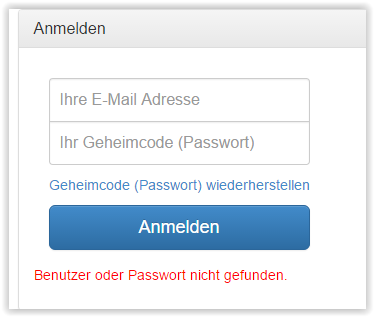
\includegraphics[width=0.5\textwidth]
		{Images/nachher_Email-und-Passwort.PNG}
		\caption{Neu umgesetzte Fehlermeldung}
	\end{figure}

	\item Wenn während einer Quiz-Teilnahme versucht wurde, das Quiz durch klicken auf den Abbrechen-Button zu verlassen, führte das teilweise zu keiner Aktion. An was dies lag, ist in folgendem Bild gut ersichtlich. Es wurde nur innerhalb der blauen Markierung auf die Klicks von Benutzer reagiert. Dieser blaue Ausschnitt war jedoch verschoben und wurde als Korrekturmassnahme direkt über dem Abbrechen-Button platziert.
	
	\begin{figure}[H]
		\centering
		
\includegraphics[width=0.75\textwidth]
		{Images/CancelButtonProblem.PNG}
		\caption{Screenshot des Problems des Abbrechen-Buttons}
		\cite{mobilequiz.ch}
	\end{figure}
	
	\begin{figure}[H]
		\centering
		
\includegraphics[width=0.75\textwidth]
		{Images/CancelButtonFix.PNG}
		\caption{Screenshot der Lösung für das Problem des Abbrechen-Buttons}
	\end{figure}
	
	\item Es wurden diverse Verbesserungen im HTML vorgenommen. Zum Beispiel waren im Registrierungsformular sämtliche Input-Typen auf 'text' gesetzt. Diese wurden entsprechend dem erwarteten Eingabetyp angepasst.
	
	Zudem wurde der Doctype-Tag von HTML4 auf HTML5 aktualisiert. Dieser Doctype-Tag teilt dem Browser mit, in welcher Version das HTML geschrieben ist und wie er das Dokument zu interpretieren hat.
	
	\item An den wichtigsten Stellen wurde die gefundene \gls{Cross-Site-Scripting} Schwachstelle behoben. Es gibt allerdings noch Stellen im Mobile Quiz an denen diese Schwachstelle nicht behoben wurde. Grundsätzlich müsste jedes Element welches von einem Benutzer (sei es Teilnehmer, Ersteller, Assistent oder Administrator) eingegeben wurde bei seiner Ausgabe so codiert werden, dass es nicht mehr ausgeführt werden kann. Wenn dies nicht gemacht ist, kann ein böswilliger Benutzer von ihm erstellten Code ausführen lassen. Dies kann im schlimmsten Fall zum Verlust von Benutzerdaten und Sessions führen. Damit kann ein Angreifer dann im Namen von anderen Benutzer im System agieren.
	
	\item Bei der Durchführung eines Quizzes wird oben links im Stil X/Y jeweils angezeigt, bei welcher Frage X der totalen Anzahl zu beantwortenden Fragen Y man sich befindet. Allerdings hatte es einen Fehler in der Logik, es wurde beim Zurück-Navigieren ebenfalls nach oben gezählt, womit die Aussage nicht mehr stimmte.
	Die Logik wurde so angepasst, dass dieser Zähler nun in jedem Fall korrekt berechnet wird. 
	
\end{itemize}


\subsection{Frage-Template}

\label{subsec:FrageTemplate}
Die Möglichkeit, Fragen offline zu erstellen und anschliessend hochzuladen, bestand bereits. Unterstützt wurde die Erfassung von Singechoice und Multiplechoice-Fragen. Dazu konnten Fragen in eine \gls{CSV}-Datei geschrieben werden. Alle korrekten Antworten wurden mit einem Asterisk (Stern-Zeichen) versehen. Eine Multiplechoice-Frage lag vor, wenn mehr als eine Antwort mit einem Asterisk versehen war.

In dieser Arbeit wurde das CSV-Template durch ein Excel-Template abgelöst. Die Gründe dazu sind die folgenden:
\begin{itemize}
	\item Die Regeln für das Erstellen waren einem kleinen Personenkreis bekannt. Sie wurden auf der Webseite nicht beschrieben. Damit die Funktion aber Verbreitung findet, muss die Vorgehensweise öffentlich zugänglich sein.
	
	Es wurde entschieden, ein Excel-Template zum Download auf der Webseite anzubieten. Darin sind alle relevanten Informationen für die Erstellung vorhanden.
	
	\item Werden die Fragen in Excel erstellt und anschliessend daraus eine CSV-Datei generiert, so hat man die Wahl zwischen 3 verschiedenen CSV-Varianten.
	
	Der Excel-Import hingegen unterstützt alle Excel-Dateien mit der Endung .xlsx. Dieses Format ist ab Excel 2007 das Standardformat und daher weit verbreitet.
	\cite{microsoft2016}
	
	\item Das CSV-Template war auf Singlechoice und Multiplechoice - Fragen beschränkt.
	
	Da neue Fragetypen unterstützt werden sollten, wurde eine neue Struktur mittels Excel erarbeitet. Um den Ersteller zu Unterstützen wurde mit Farben und weiteren Funktionen gearbeitet, welche durch CSV nicht unterstützt werden.

\end{itemize}

Durch den Einsatz des neuen Templates konnte auch ein Umlaute-Bug behoben werden, welcher aufgrund des CSV-Templates entstand. Bei der Erstellung von Fragen wird geprüft, ob die gleiche Frage bereits schon besteht. Falls dies der Fall ist, wird beim Quiz die bestehende Frage hinzugefügt und keine neue erstellt. Mit dem CSV-Template gab es einen Fehler bei der Erkennung von Umlauten, wodurch es zu Doppel-Erstellungen kam. Mit dem neuen Excel-Template geschieht dies nicht mehr.

\bigskip

Ein Beispiel des ursprünglichen Formats sowie des neuen Excel-Templates ist im Anhang, im Kapitel 19 \glqq Details zur Lösungsfindung\grqq auf den Seiten \hyperlink{page.\getpagerefnumber{pdf:csvTemplate}}{\getpagerefnumber{pdf:csvTemplate}} und \hyperlink{page.\getpagerefnumber{pdf:excelTemplate}}{\getpagerefnumber{pdf:excelTemplate}}, ersichtlich.

\bigskip

Der neue Template-Import wurde mit PHPExcel \cite{phpexcel} umgesetzt. Diese PHP-Library war bereits im Projekt eingebunden und wird dazu verwendet, die Rangliste aller Teilnehmenden eines Quizzes in eine Excel-Datei zu Exportieren. Die neue Logik befindet sich hauptsächlich in der neu erstellen Datei \glqq importExcel.php\grqq.

\bigskip

Bei PHPExcel gab es bis zur Version 1.7.9 eine \gls{XML External Entitiy} - \gls{Vulnerability}. Dadurch war es Remote-Angreifern möglich, beliebige Dateien auf dem Server zu lesen oder eine \gls{Denial of Service} - Attacke durchzuführen. \cite{cvedetails_phpexcel}
Da bei Mobile Quiz allerdings die Version 1.8.0 verwendet wird, ist dies nicht mehr möglich. Es wurde mit dem Wissen aus dem Fach Informationssicherheit 3 versucht eine solche Attacke durchzuführen, was ebenfalls zum Ergebnis führte, dass diese Sicherheitslücke nicht mehr vorhanden ist.



\subsection{Ablauf Quiz-Erstellung}
\label{subsec:quiz-erstellung}

Um in Mobile Quiz ein Quiz zu erstellen war es bisher so, dass zuerst die Fragen und anschliessend das Quiz separat erstellt werden musste. Dieser Ablauf war nicht nur bei der eigenen Untersuchung der Webseite unklar, er warf auch bei den Usability-Tests Fragen auf. Dabei versuchten die Teilnehmer oft ein Quiz zu erstellen und wollten darin die Fragen erfassen. Da dies auch der Standard-Ablauf aller anderen untersuchten Quiz-Webseiten war, wurde er auch in Mobile Quiz implementiert.

Wie auf der unteren Abbildung ersichtlich ist, werden nun zuerst die allgemeinen Informationen erfasst, welche bei jeder Quiz-Durchführung gleich sein sollen. Anschliessend können im Frage-Tab neue Fragen erstellt oder bestehende zum Quiz hinzugefügt werden. Schliesslich können eine oder mehrere Durchführungen erstellt werden.

\begin{figure}[H]
	\centering
	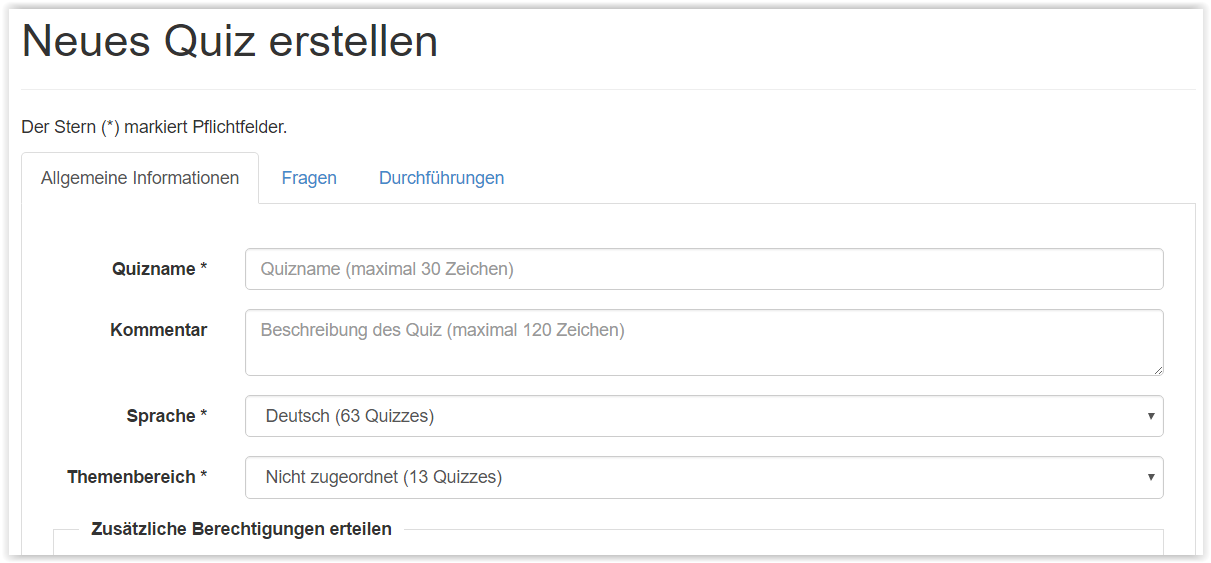
\includegraphics[width=0.8\textwidth]{Images/Quiz_Erstellen1.PNG}
	\caption{Neuer Ablauf der Quiz-Erstellung}
\end{figure}

Das Konzept der Durchführungen wurde in diesem Projekt neu erarbeitet und entstammte aus dem Wunsch, Quizzes für die einzelnen \acrshort{CN1}-Praktikumsgruppen anzupassen. Dabei nehmen die Studenten, in immer der gleichen Gruppe, jeweils im zwei-Wochen-Takt am Praktikum teil. Es gibt sowohl in der ersten als auch in der zweiten Woche mehrere Praktikumsgruppen.

Nach dem Praktikums wird das Gelernte mit einem Online-Quiz überprüft. Dieses soll aber erst nach dem Praktikum und nur eine Woche lang aufgeschaltet sein. Dies konnte mit der bestehenden Mobile Quiz - Version nur mit Mehraufwand umgesetzt werden, da der festgelegte Durchführungszeitraum für alle Gruppen gleich war. Unterschiedliche Termine konnten nur festgelegt werden, indem mehrere Quizzes mit entsprechenden Datumsbeschränkungen erstellt wurden.

\bigskip\bigskip

\textbf{Lösung}
\bigskip

Neu ist es für solche Fälle möglich, ein Quiz mit mehreren Durchführungen zu erstellen. Das Quiz selbst umfasst nur noch Eigenschaften wie der Name oder die Sprache, welche bei jeder Durchführung gleich sind. Ebenfalls werden die Fragen mit dem Quiz verknüpft. Anschliessend ist es möglich, für das Quiz mehrere, unterschiedliche Durchführungen zu erstellen. Diese beinhalten Einstellungen wie zum Beispiel den Start- und Endzeitpunkt sowie die zugewiesenen Gruppen und Teilnehmer.


\begin{figure}[H]
	\centering
	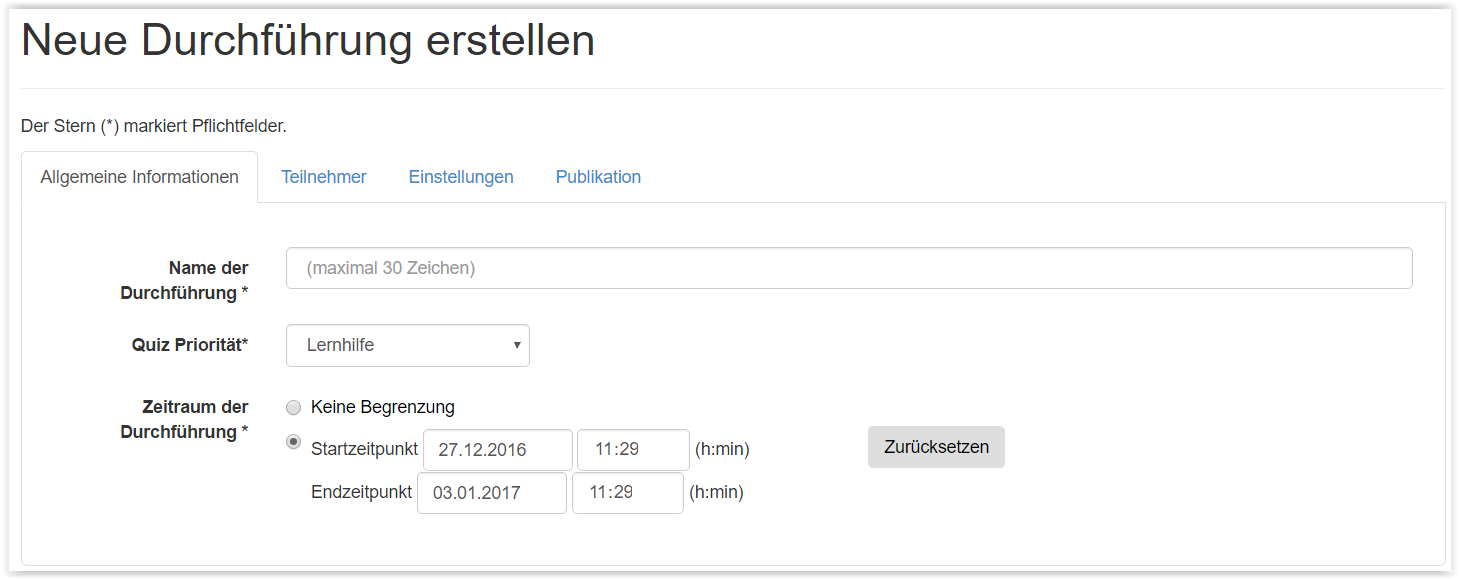
\includegraphics[width=0.8\textwidth]{Images/Quiz_Durchfuehrung1.PNG}
	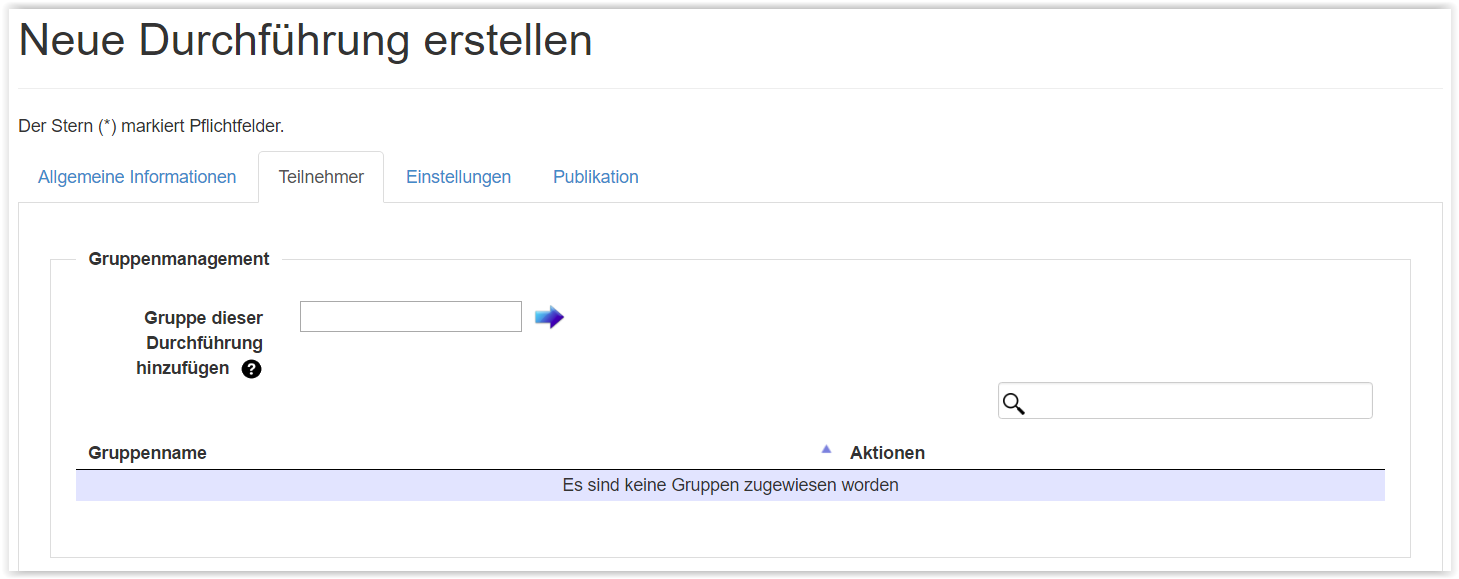
\includegraphics[width=0.8\textwidth]{Images/Quiz_Durchfuehrung2.PNG}
	\caption{Erfassung einer Durchführung}
\end{figure}


Auf diese Weise bietet Mobile Quiz für die oben beschriebene Situation eine einfache Lösung an. Das Quiz selbst muss nur noch einmal erstellt werden. Für die Praktikumsgruppen der ersten Woche wird dann eine Durchführung für den Zeitraum einer Woche nach dem Praktikum erfasst und die Gruppen zugewiesen. Das gleiche gilt für die Praktikumsgruppe der zweiten Woche. \\

\bigskip\bigskip

\textbf{Weitere Vereinfachungen}
\bigskip

Mobile Quiz geht hier allerdings noch einen Schritt weiter. Schon in der bestehenden Version gab es drei Quiz-Prioritäten, nämlich Lernhilfen für Unterrichtsfragen, Lernkontrollen für Testate und Prüfungen. Jede dieser Prioritäten besitzt bereits vordefinierte Einstellungen, welche automatisch gesetzt werden, wenn bei der Quiz-Erstellung die Priorität gewechselt wird. So ist zum Beispiel die maximale Anzahl Teilnahmen bei einer Prüfung immer eins. Somit wird der Ersteller davon befreit, alle Einstellungsmöglichkeiten selbst zu setzen. Möchte er trotzdem einzelne Werte verändern, so werden diese neuen Werte in der Datenbank in seinem Profil abgespeichert. Bei jeder nachfolgenden Quiz-Erstellung wird dann geprüft, ob beim Ersteller solche Werte gespeichert sind. Falls dies nicht der Fall ist, werden wieder die vordefinierten Default-Werte verwendet. Die mit Herr Heinzmann besprochenen Default-Werte sind im Anhang unter \glqq Default-Einstellungen\grqq auf Seite \hyperlink{page.\getpagerefnumber{pdf:defaultEinstellungen}}{\getpagerefnumber{pdf:defaultEinstellungen}} ersichtlich.

\bigskip\bigskip

Aufgrund von fehlender Zeit konnte die Implementierung der Durchführungs-Erstellung nicht abgeschlossen werden. Dieser Punkte wurde deshalb in den noch nicht fertiggestellten Arbeiten \ref{subsec:NichtFertiggestellteArbeiten} aufgeführt.





\subsection{Design Quiz- und Frage-Erstellung}
Bei der ersten Durchführung der \gls{Usability-Test}s stellte sich heraus, dass die Teilnehmer von den Einstellungsmöglichkeiten teilweise überfordert waren. Dies lag vor allem daran, dass sehr viele Optionen auf einmal angezeigt wurden und diese zudem unstrukturiert, auf der ganzen Seite verteilt, dargestellt wurden.


\begin{figure}[H]
	\centering
	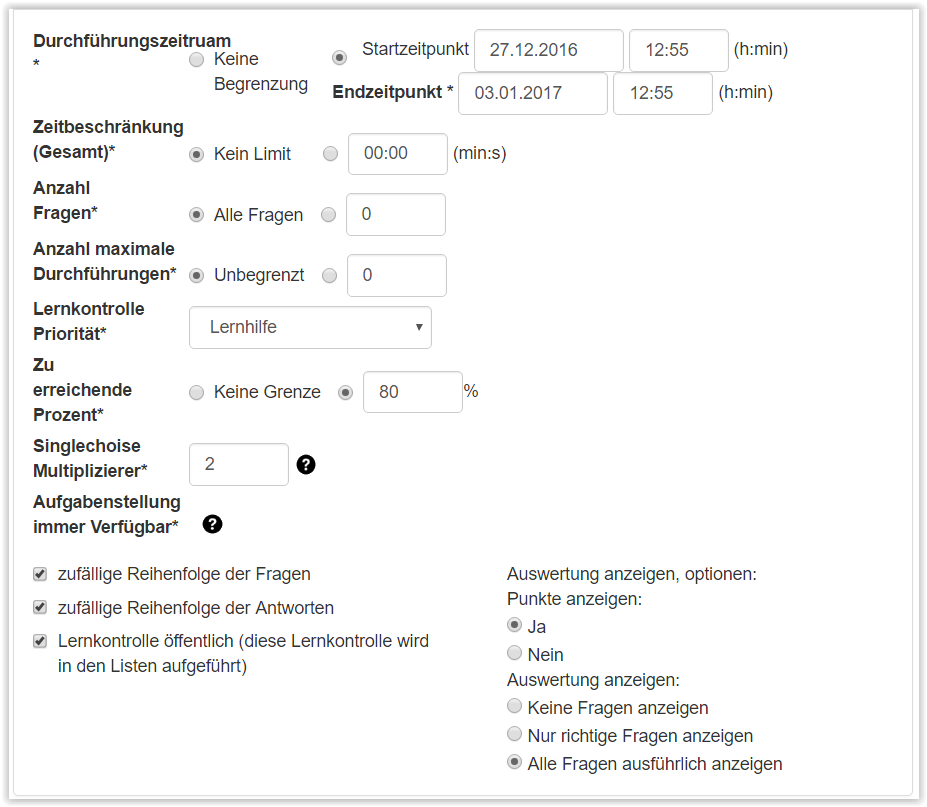
\includegraphics[width=0.6\textwidth]{Images/Einstellungen_alt.PNG}
	\caption{Einstellungsmöglichkeiten der bestehenden Mobile Quiz - Version 3}
	\cite{mobilequiz.ch}
\end{figure}


Um dem entgegenzuwirken wurde die Quiz-Erstellung auf mehrere Seiten aufgeteilt, welche thematisch zusammengehören. Diese Seite werden in einzelnen Tabs dargestellt. Da Tabs auf mobilen Geräten nicht immer gut dargestellt werden, wurde ein Design gesucht, welches die Inhalte in dieser Ansicht optimal anzeigt. Dieses wurde mit dem Accordion-Design gefunden.


\begin{figure}[H]
	\centering
	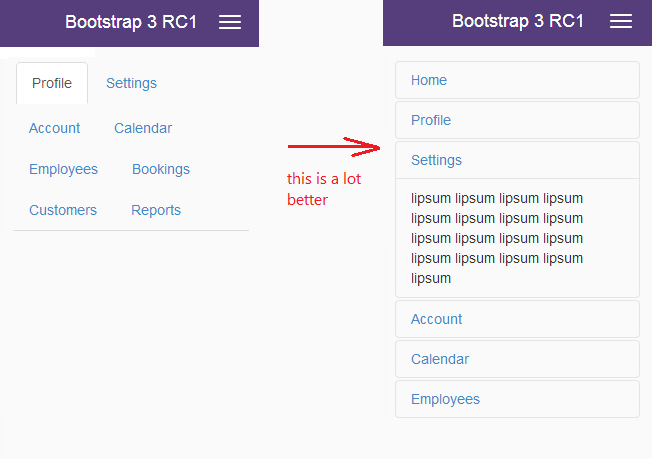
\includegraphics[width=0.6\textwidth]{Images/Bootstrap_Accordion.png}
	\caption{Tabs im Vergleich zum Accordion - Design}
	\cite{tabs_accodion}
\end{figure}

Um nun beide Ansichten zu vereinen wurde \glqq Bootstrap Tab Collapse\grqq \cite{bootstrap-tabcollapse} verwendet. Das Design verhält sich wie folgendermassen:

Bis zu einer gewissen Fensterbreite werden die Inhalte mit Tabs angezeigt. Bei kleineren Bildschirmen wird automatisch in die Accordion-Ansicht gewechselt. Dieses verdankt seinen Namen den aufklappenden und zusammenziehenden Elementen, welche es wie ein Akkordeon aussehen lassen.

Somit konnten die Seiteninhalte für die Quiz-Erstellung auf mehrere Seiten verteilt werden, welche in jeder Ansicht gut dargestellt werden können.


\begin{figure}[H]
	\centering
	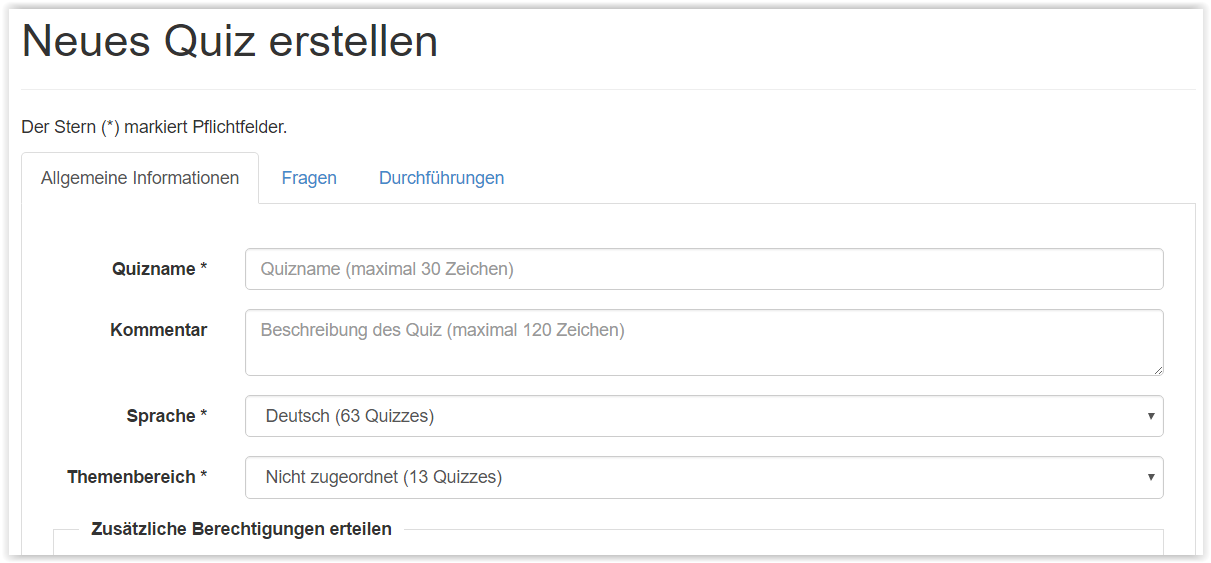
\includegraphics[width=0.8\textwidth]{Images/Quiz_Erstellen1.PNG}
	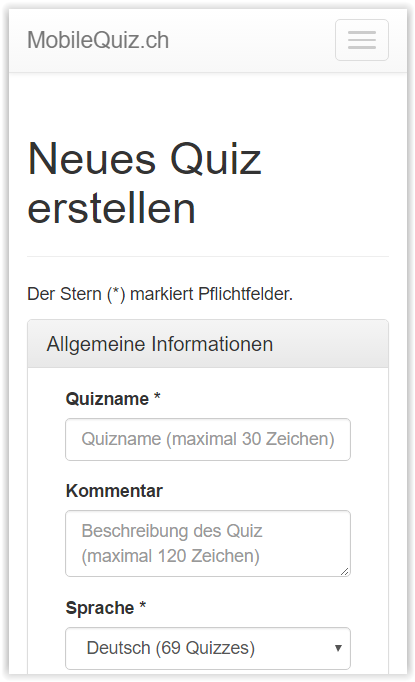
\includegraphics[width=0.3\textwidth]{Images/Quiz_Erstellen_Mobile.PNG}
	\caption{Desktop- und Mobile-Ansicht der Quiz-Erstellung}
\end{figure}

\bigskip
\textbf{Funktionale Umstellungen}
\bigskip

Da nun mit dem Quiz zusammen auch Fragen und Durchführungen erstellt werden, dauert dieser Vorgang länger als das alleinige Erfassen eines Quizzes in der bestehenden Mobile Quiz - Version. Da es sein kann, dass der Benutzer diesen Vorgang unterbrechen muss, beispielsweise arbeitet er im Zug und muss umsteigen, sollten die Benutzereingaben zwischendurch gespeichert werden.

Für die Umsetzung wäre ein halb-minütiger Countdown möglich gewesen, bei dessen Ablauf alle Daten im Hintergrund an den Server geschickt werden. Die Probleme liegen darin, dass der Ersteller im schlimmsten Fall 29 Sekunden Arbeit verliert oder unnötig viele Daten verschickt werden, falls keine oder nur wenige Änderungen vorliegen.

Aus diesem Grund wurde entschieden, jede neue Benutzereingabe einzeln an den Server zu senden. Dies wird mit \acrfull{AJAX} umgesetzt, welches es ermöglicht Daten an den Server zu schicken, ohne die gesamte Seite neu zu laden. Da jeweils nur ein Eingabefeld verändert wird, werden jeweils nur die wirklich benötigten Daten an den Server geschickt. Zudem ist die Handhabung auf dem Server ebenfalls einfacher, da meist nur ein Attributwert eines einzelnen Datenbank-Eintrages verändert werden muss.

Damit ein Benutzer weiss, dass seine Eingabedaten fortlaufend gespeichert werden, bekommt er jedes Mal eine entsprechende Meldung zurück. In Abbildung \ref{fig:Eingabe bei der Quiz-Erstellung} ist links ersichtlich, wie eine solche Meldung aussieht und rechts was der entsprechende \acrshort{AJAX}-Request an den Server beinhaltet.


\begin{figure}
	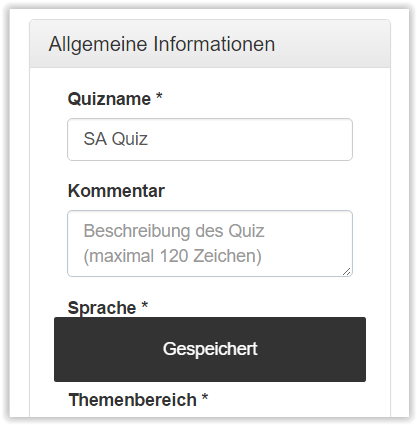
\includegraphics[width=0.35\textwidth]{Images/Quiz_Erstellen_Gespeichert.PNG}
	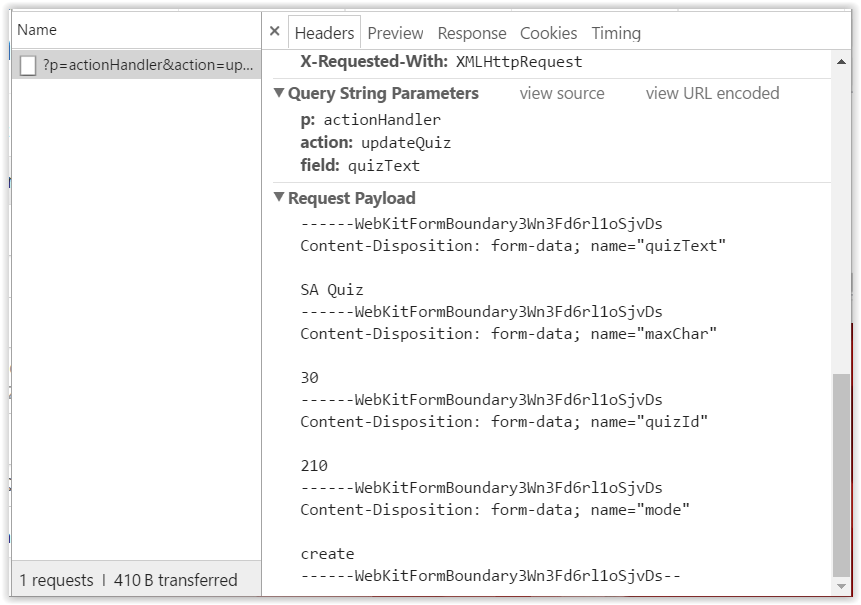
\includegraphics[width=0.65\textwidth]{Images/Quiz_Erstellen_Request.PNG}
	\caption{Eingabe bei der Quiz-Erstellung}
	\label{fig:Eingabe bei der Quiz-Erstellung}
\end{figure}

\bigskip\bigskip

\textbf{Frage-Erstellung}

\bigskip

Das oben beschriebene Design und die Kommunikation mit \acrshort{AJAX} wurde ebenfalls für die Frage-Erstellung umgesetzt. Dabei waren die Überlegungen die gleichen. \\

Zusätzlich wurde implementiert, dass eine Frage erst mit der ersten Benutzereingabe erstellt wird. Will sich ein Ersteller die Eingabemaske nur ansehen, so werden noch keine Daten in die Datenbank gespeichert.

Schliesslich wurde ein weiteres Verhalten implementiert, welches das Erfassen der Frage vereinfacht. Wenn ein Ersteller überprüfen will, ob seine Daten wirklich gespeichert wurden, so aktualisiert er die Seite und es wird normalerweise seine letzte angeforderte Seite erneut geladen. Dies ist in diesem Fall aber die Frage-Erstellungs-Seite, welche ihm ein neues, leeres Erfassungsformular anzeigt. Damit aber seine soeben eingegebenen Daten angezeigt werden, wurde mit JavaScript der \glqq Unload-Event\grqq abgefangen, welcher durch eine Seitenaktualisierung ausgelöst wird, und die angefragte \gls{URL} ausgetauscht, sodass neu die Frage-Bearbeitungs-Seite vom Server geladen wird.
Dieses Verhalten funktioniert bisher allerdings nur in Firefox \cite{firefox}.



\subsection{Umgestaltung Startseite Teilnehmer / Ersteller}

Die Startseite enthält neu nicht mehr die einzelnen Quizzes, sondern alle Durchführungen der Quizzes. Diese Umstellung war nötig, damit Teilnehmer ihre Durchführung leicht finden und nicht zuerst über das Quiz einsteigen müssen.

Wie im Abschnitt Interessensgruppen und Filterumstellung \ref{InteressensgruppenUndFilterumstellung} beschrieben, wurde ausserdem der Filter so angepasst, dass neu eine Mehrfachauswahl von Optionen möglich ist.

\bigskip\bigskip

\begin{quote}
	\glqq Probleme bereitete meist, dass Funktionen nicht auf den ersten Blick ersichtlich sind.\grqq
\end{quote}

Dies war eine der Schlussfolgerung des ersten \gls{Usability-Test}s und bezog sich vor allem auf die Startseite, da von dort aus die meisten Aktionen gestartet werden können. In dieser Arbeit wurde das Problem so angegangen, dass einerseits weniger Informationen zu den einzelnen Quizzes angezeigt werden und andererseits die Icons durch Text ergänzt wurden.

Konkret wurde die Anzahl Fragen, die Anzahl eigene Teilnahmen sowie die Anzahl Gesamtteilnahmen entfernt. Der Benutzer kann somit schneller die benötigten Informationen erfassen. Um die korrekte Durchführung zu finden war es jedoch nötig, zusätzlich den Durchführungstyp aufzuführen. 


\begin{figure}[H]
	\centering
	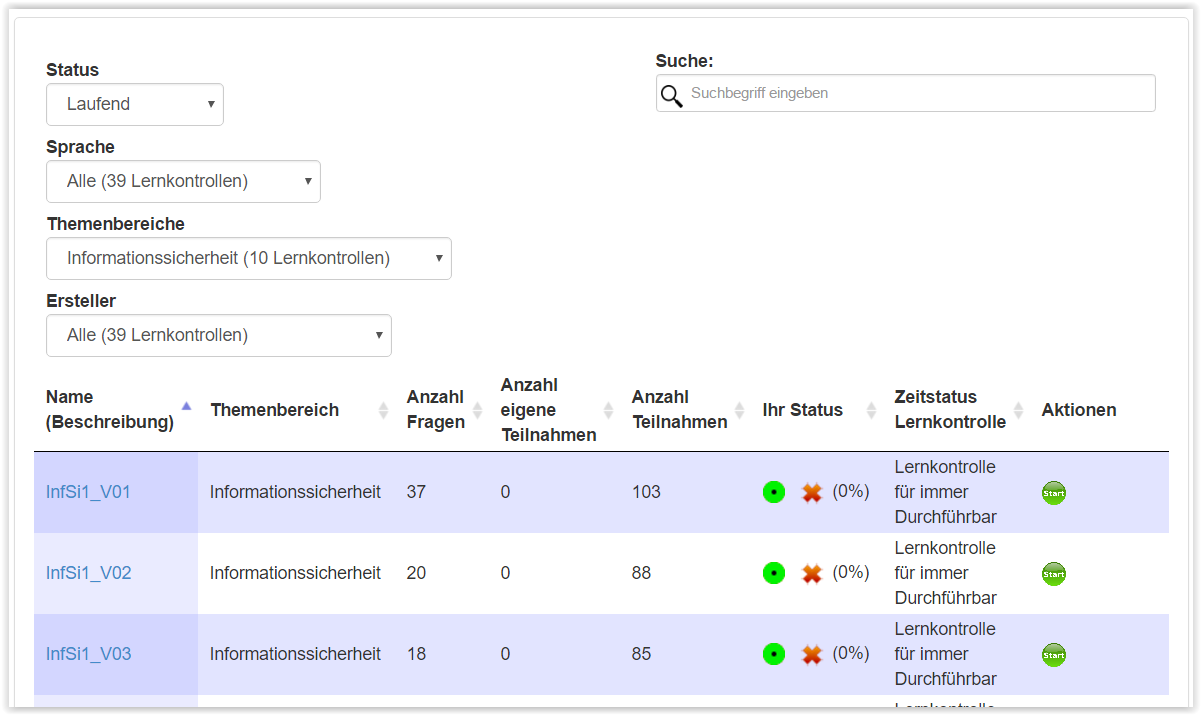
\includegraphics[width=0.8\textwidth]{Images/Startseite_alt.PNG}
	\caption{Startseite der bestehenden Mobile Quiz - Version 3}
	\cite{mobilequiz.ch}
\end{figure}


\begin{figure}[H]
	\centering
	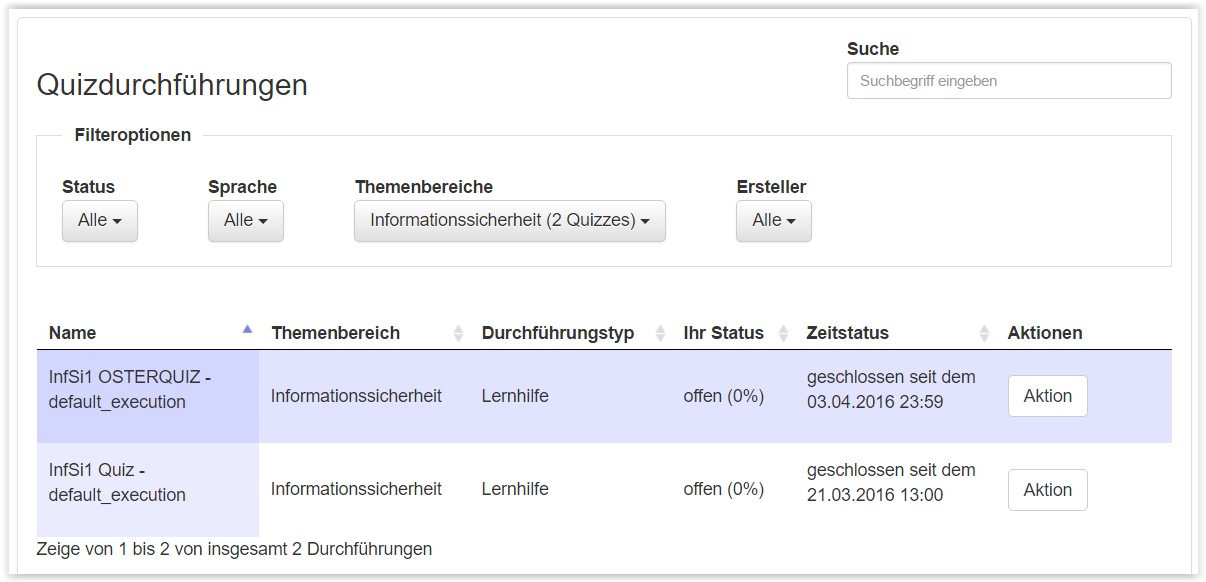
\includegraphics[width=0.8\textwidth]{Images/Startseite_neu.PNG}
	\caption{Neue Startseite für den Teilnehmer}
\end{figure}


Weiter wurden die unterschiedlichen Icons der Aktionen durch ein ausklappbares Menu ersetzt. Dieses beinhaltet die Aktionen als Text sowie einheitliche Icons. Dazu wurden Glyphicons von Bootstrap \cite{glyphicons} verwendet. Dies vereinfacht das Navigieren für den Benutzer, da er alle Aktionen beschrieben sieht und nicht, wie zuvor, erst mit der Maus über alle Symbole fahren muss. Dieses Verhalten war auf mobilen Geräten zudem gar nicht möglich, da es dort den \glqq Mouse-Hover-Effekt\grqq, also das darüberfahren mit der Maus, gar nicht gibt. Die neue Lösung ist somit auch mobile-tauglich.

Icons gibt es zwar weiterhin, diese dienen aber dem schnelle Erfassen der Auswahlmöglichkeiten und der Gruppierung von ähnlichen Aktionen.


\begin{figure}[H]
	\centering
	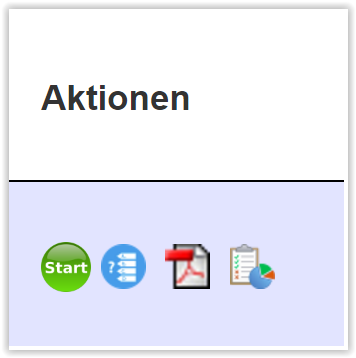
\includegraphics[width=0.3\textwidth]{Images/Aktionen_alt.PNG}
	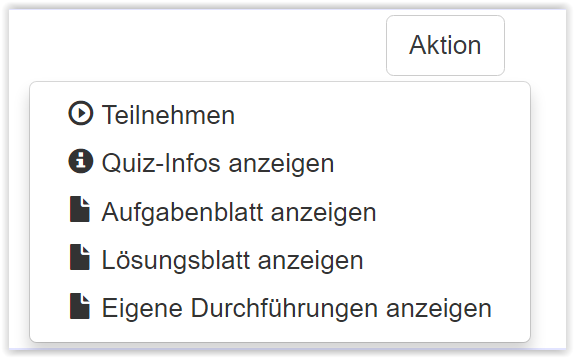
\includegraphics[width=0.5\textwidth]{Images/Aktionen_neu.PNG}
	\caption{Vergleich des bestehenden und der neuen Aktions-Anzeige}
	\cite{mobilequiz.ch}
\end{figure}







\section{Neuerungen}

\subsection{Fragen mit Bilder}

\subsubsection{Hochladen und Entfernen eines Bildes}
Bei jedem Fragetyp ist es neu möglich ein Bild zu hinterlegen. Die Funktion des Bild-Uploads auf den Server bestand bereits, wurde aber erweitert.
\\
\\
Beim Hochladen des Bildes wurde zuvor eine Fehlermeldung ausgegeben, wenn ein Bild eine Grösse von über 20 Megabyte überstieg. Diese Limite wurde herabgesetzt, weil ein Bild von dieser Grösse zu lange benötigt, bis es heruntergeladen werden kann. Unten ist ein Vergleich von Downloadzeiten bei verschiedenen Dateigrössen aufgeführt. Die angegebene Geschwindigkeit ist die Downloadgeschwindigkeit welche 80\% der Kunden erreichen. Diese wurden anhand von Speedtests der cnlab AG \cite{cnlab_speedtest} ermittelt. \\


\begin{tabular}{|c|c|c|c|}
	\hline 
	Dateigrösse & Art & Downloadgeschwindigkeit & Benötigte Zeit \\ 
	\hline 
	20 MB & DSL-Anbieter & 13,6 Mbit/s & 11,8 s \\ 
	\hline 
	20 MB & Kabel-Anbieter & 40,6 Mbit/s & 3,9 s \\ 
	\hline 
	20 MB & Mobile & 8,9 Mbit/s & 18 s \\ 
	\hline 
	5 MB & DSL-Anbieter & 13,6 Mbit/s & 2,9 s \\ 
	\hline 
	5 MB & Kabel-Anbieter & 40,6 Mbit/s & 1 s \\ 
	\hline 
	5 MB & Mobile & 8,9 Mbit/s & 4,5 s \\ 
	\hline 
	800 KB & DSL-Anbieter & 13,6 Mbit/s & 0,5 s \\ 
	\hline 
	800 KB & Kabel-Anbieter & 40,6 Mbit/s & 0,2 s \\ 
	\hline 
	800 KB & Mobile & 8,9 Mbit/s & 0,7 s \\ 
	\hline 
\end{tabular}\\

Falls ein Bild nun 800 Kilobyte übersteigt, so wird es so lange komprimiert, bis seine Dateigrösse darunterliegt. Dies wird durch die PHP-Funktion 'imagecopyresampled' erreicht. Als Code-Vorlage diente das Beispiel von www.williseiler.ch \cite{willis_php}. \\

Weiter gibt es Grössenbeschränkungen von Apache selbst \cite{stackoverflow_largeFilePHP}. Im File 'php.ini' können folgende drei Werte definiert werden:
\begin{itemize}
	\item upload\_max\_filesize: Legt die maximale Dateigrösse für eine Upload-Datei fest. Der Standardwert liegt bei 2 MB.
	\item post\_max\_size: Legt die maximale Grösse aller POST-Daten zusammen fest. Der Standardwert liegt bei 8 MB.
	\item max\_file\_uploads: Legt die maximale Anzahl aller Dateien fest, welche auf einmal hochgeladen werden können. Der Standardwert liegt bei 20 Dateien.
\end{itemize}

Werden via Excel-Template 10 Fragen mit je einem Bild à 1 Megabyte hochgeladen, so ist dies mit der Standardkonfiguration nicht möglich. Diese wurde deshalb folgendermassen angepasst:
\begin{itemize}
	\label{php.ini:neueGroessenbeschraenkungen}
	\item upload\_max\_filesize: Neu 5 MB. Grössere Dateien benötigen zu lange für den Upload. Allerdings soll der Benutzer nicht nur auf kleine Grössen beschränkt sein, deshalb wurde von der 2MB-Standardgrösse abgewichen.
	\item post\_max\_size: Neu 25 MB. Bei dieser Grösse beträgt die Uploadzeit bei einer Geschwindigkeit von 10,3 Mbit/s 19,4 Sekunden. Dies ist die Uploadgeschwindigkeit von 80\% der DSL-Messungen, welche beim Speedtest der cnlab AG \cite{cnlab_speedtest} erreicht wurde. Dem Benutzer sollte bewusst sein, dass der Upload bei so vielen Dateien einige Zeit in Anspruch nimmt.
	Auf der anderen Seite soll der Benutzer aber auch nicht eingeschränkt werden. Es soll möglich sein, gleichzeitig 20 Fragen mit Bildern à 1 MB sowie 1 Frage mit einem grösseren Bild plus das Excel-Template hochzuladen.
	\item max\_file\_uploads: Neu 25 Dateien. Der Standard-Wert wird nur leicht angehoben, da es möglich sein soll 20 Fragen mit Bildern gleichzeitig zu erstellen. Damit würde das Maximum von 20 Dateien nicht ausreichen.
\end{itemize}

Das Excel-Template für die Frage-Erstellung wurde ebenfalls erweitert, so dass auch Fragen mit Bilder erstellt werden können. Dazu wurde eine neue Spalte eingefügt, bei welcher man den Bildnamen inklusive Endung einträgt. Die Bilder müssen sich dabei im gleichen Ordner wie das Template befinden. Anschliessend wird der gesamte Ordner hochgeladen.

Es war dabei nicht möglich, nur die Excel-Datei alleine hochzuladen und anschliessend die Bilder selbstständig zu holen. Dies wäre bezüglich der Sicherheit höchst bedenklich.


\subsubsection{Anzeige eines Bildes}
Das Bild sollte beim Anzeigen der Frage gross genug dargestellt werden. Auf dem Computer war dies kein Problem, da ein Browserfenster genug Platz dazu bot, bei einem Smartphone hingegen war dieser beschränkt. Deshalb wurde die Anzeige so umgesetzt, dass das Bild beim Klick darauf auf dem ganzen Bildschirm dargestellt wird. Dies wurde mit Photoswipe \cite{photoswipe} umgesetzt, welches von GitHub \cite{github_photoswipe} bezogen wurde. Photoswipe ist eine JavaScript-Library, welche es ermöglicht, Bildgalerien auf Websites darzustellen. Sie unterstützt unter anderem Touch-Gesten und Zoom. So ist es kein Problem, ein Bild mit vielen Details darzustellen.

\begin{figure}
	\centering
	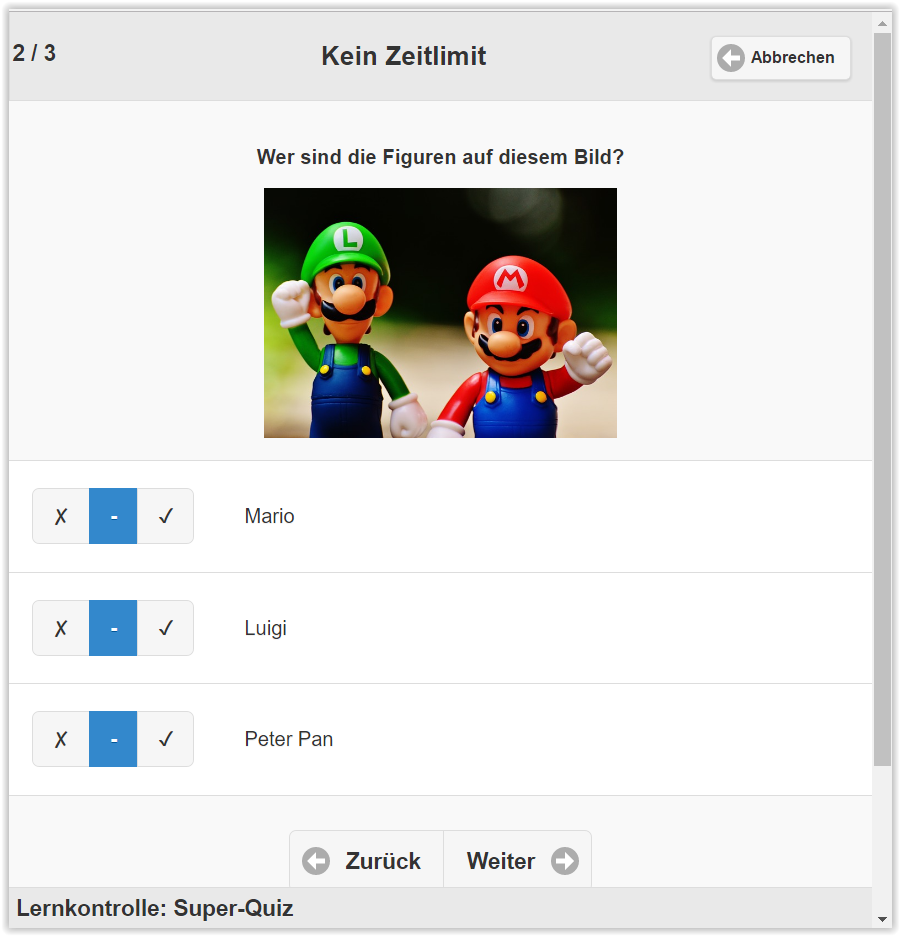
\includegraphics[width=0.5\textwidth]{Images/Frage-Bild_Anzeige_PC.PNG}
	\caption{Anzeige des Frage-Bildes am Computer}
	Quelle Fragebild: \cite{_bild_pixabay_mario_}
\end{figure}

\begin{figure}
	\centering
	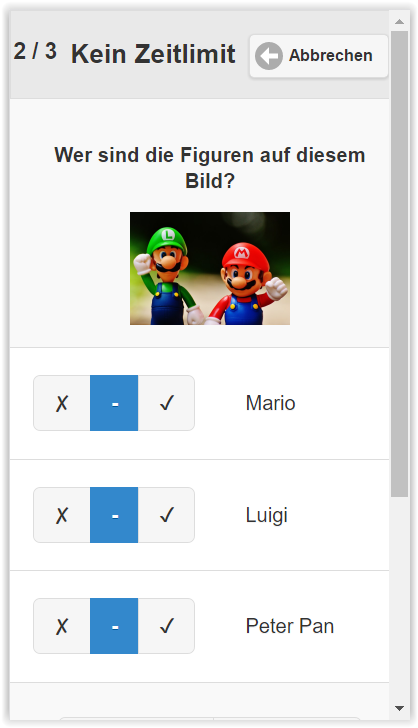
\includegraphics[width=0.3\textwidth]{Images/Frage-Bild_Anzeige_Mobile.PNG}
	
\includegraphics[width=0.3\textwidth]{Images/Frage-Bild_Anzeige_Mobile_Full.PNG}
	\caption{Anzeige des Frage-Bildes auf dem Smartphone}
	Quelle Fragebild: \cite{_bild_pixabay_mario_}
\end{figure}

Da sich eine Frage, bei welcher ein Bild hochgeladen wird, oft auf Inhalte aus dem Bild bezieht, wurde auch für die Auswertungsseite eine Bild-Anzeige implementiert. Somit können die Auswertungen besser nachvollzogen werden.

Weiter wurde die Generierung des PDF-Aufgabenblattes und Lösungsblattes ergänzt, damit auch dort die Bilder angezeigt werden. Hat man unterwegs kein Internet, so kann man sich die Fragen damit auch vorgängig herunterladen und im Zug anschauen.








\newpage
\subsection{Feedback an Quiz-Ersteller}
Bei der Ausarbeitung der neuen Fragetypen kam die Idee einer Freitext-Frage auf. Bei diesem Fragetyp sind keine Antwortmöglichkeiten vorgegeben, stattdessen schreibt der Teilnehmer seine Antworten in ein leeres Textfeld. Das Problem dabei ist aber die Korrektur, da eine korrekte Antwort auf viele verschiedene Wege niedergeschrieben werden kann. Aus diesem Grund wurde beschlossen, diesen Fragetyp nicht umzusetzen, aber die Idee andernorts zu verwenden.

Ist eine Frage unklar gestellt, gibt es Schreibfehler oder andere Verbesserungsmöglichkeiten, so musste dies ein Teilnehmer bis anhin selbst notieren und den Quiz-Ersteller, in den meisten Fällen der Dozent, im Unterricht fragen. Dies setzt aber voraus, dass der Quiz-Ersteller für den Teilnehmer immer ansprechbar ist. Erstellt ein Dozent aus Rapperswil ein Quiz, an welchem Teilnehmer der ganzen Schweiz mitmachen, so besteht diese Möglichkeit nicht.

Dieses Problem wurde nun angegangen. Unter jeder Frage gibt es neu die Möglichkeit einen Kommentar direkt an den Quiz-Ersteller zu senden.

\begin{figure}[H]
	\centering
	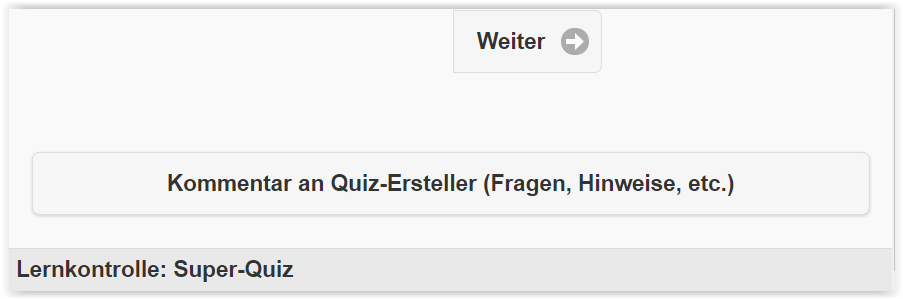
\includegraphics[width=0.7\textwidth]{Images/Feedback-Button.PNG}
	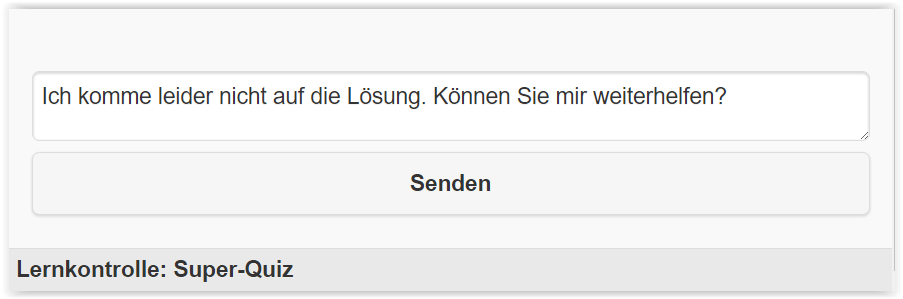
\includegraphics[width=0.7\textwidth]{Images/Feedback-Frage.PNG}
	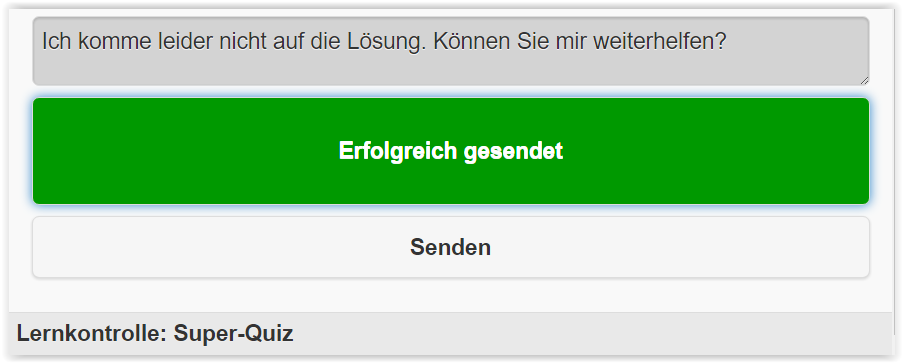
\includegraphics[width=0.7\textwidth]{Images/Feedback-Frage-gesendet.PNG}
	\caption{Ablauf der Feedback-Erfassung}
\end{figure}


Nach dem Senden des Feedbacks erhält der Quiz-Ersteller eine E-Mail. Darin ist nicht nur die Frage des Teilnehmers aufgeführt, sondern auch Informationen zum Teilnehmer selbst sowie die gesamte Frage inklusive Antwortmöglichkeiten. Somit hat der Quiz-Ersteller alle Informationen, um auf die Teilnehmer-Frage zu antworten.

\begin{figure}[H]
	\centering
	
\includegraphics[width=0.9\textwidth]{Images/Feedback-Mail_Quiz-Ersteller.PNG}
	\caption{E-Mail an Quiz-Ersteller}
\end{figure}

Der Teilnehmer selbst erhält ein Bestätigungsmail mit den gleichen Informationen, wie sie auch der Quiz-Ersteller erhält.

\begin{figure}[H]
	\centering
	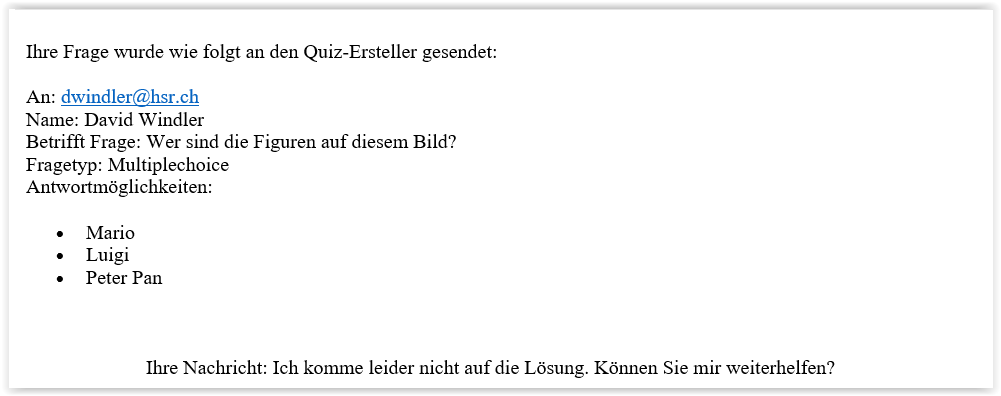
\includegraphics[width=0.9\textwidth]{Images/Feedback-Mail_Teilnehmer.PNG}
	\caption{Bestätigungs-E-Mail an Teilnehmer}
\end{figure}




\subsection{Interessensgruppen und Filterumstellung}
\label{InteressensgruppenUndFilterumstellung}
Loggt sich ein Teilnehmer bei Mobile Quiz ein, so soll er möglichst wenige Klicks von seinem zu lösenden Quiz entfernt sein. Dadurch spart er Zeit da, er sich nicht mit Filteroptionen und Suchfeldern auseinandersetzen muss. Doch wie erkennt Mobile Quiz welche Quizzes für den Teilnehmer interessant sind?

Möglich wäre es nachzuschauen, zu welchem Themengebiet der Teilnehmer schon Quizzes gelöst hat und aufgrund dessen die Filterauswahl bereits auf das Themengebiet mit seinen meisten Teilnahmen zu setzen. Das Problem dieser Methode liegt darin, dass sie für neu registrierte Teilnehmer nicht verwendet werden kann.
Aus diesem Grund wurde eine noch einfachere Methode implementiert. Dabei wird bei der Registrierung eines oder mehrere Interessengebiete angegeben. Diese werden dabei vorgemerkt und beim anschliessenden Aufruf aller Durchführungen wird der Themengebiet-Filter entsprechend der Interessensgebiete des Teilnehmers gesetzt. Meldet sich beispielsweise ein Student von \acrshort{CN1} bei Mobile Quiz an und setzt das Interessengebiet entsprechend, so werden zuerst immer die Quiz-Durchführungen von \acrshort{CN1} angezeigt. Besucht er zu einem späteren Semester das Modul Informationssicherheit 1, so kann er das Interessensgebiet jederzeit in seinen Profileinstellungen ändern.

\begin{figure}[H]
	\centering
	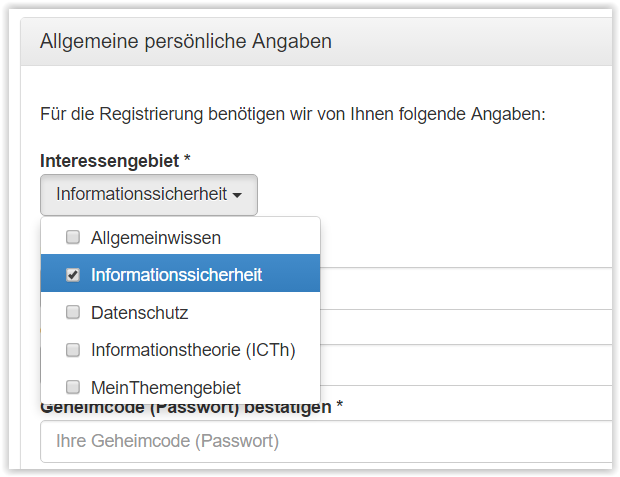
\includegraphics[width=0.5\textwidth]{Images/Themengebiet_Angabe_Registrierung.PNG}
	\caption{Angabe des Interessengebietes bei der Registrierung}
\end{figure}

Wie werden die Interessen der Teilnehmer in der Datenbank abgespeichert? Dazu half die Umstellung der Datenbank, welche es nun zulässt, dass ein Teilnehmer in mehreren Gruppen eingetragen werden kann.
Für jedes Themengebiet wurde eine Interessengruppe erstellt. Gibt ein Teilnehmer ein neues Interesse an, so wird er automatisch zur entsprechenden Interessen-Gruppe hinzugefügt. Interessengruppen werden automatisch mit der Erfassung eines neuen Themengebietes erstellt, beziehungsweise mit dem Entfernen wieder gelöscht und alle Teilnehmer ausgetragen.

\bigskip

Damit ein Teilnehmer mehrere Interessensgebiete angeben kann, war es nötig die Implementierung der Filter zu ändern. Bisher konnte jeweils nur eine Auswahl pro Filter gesetzt werden. Für die Umsetzung wurde die Library 'Bootstrap Multiselect' \cite{bootstrap_multiselect} von David Stutz verwendet. Durch eine Logikumstellung auf dem Server war es anschliessend für Quiz-Durchführungen und Fragen möglich eine Mehrfachauswahl pro Filter zu setzen.

\begin{figure}[H]
	\centering
	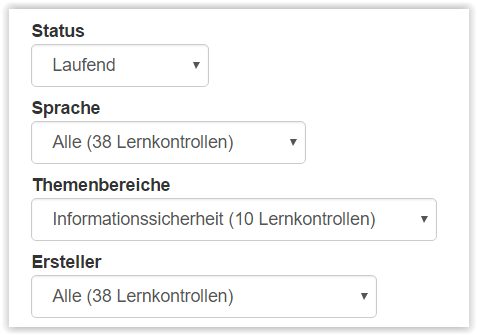
\includegraphics[width=0.462\textwidth]{Images/Alte_Filter_Mobile_Quiz.PNG}
	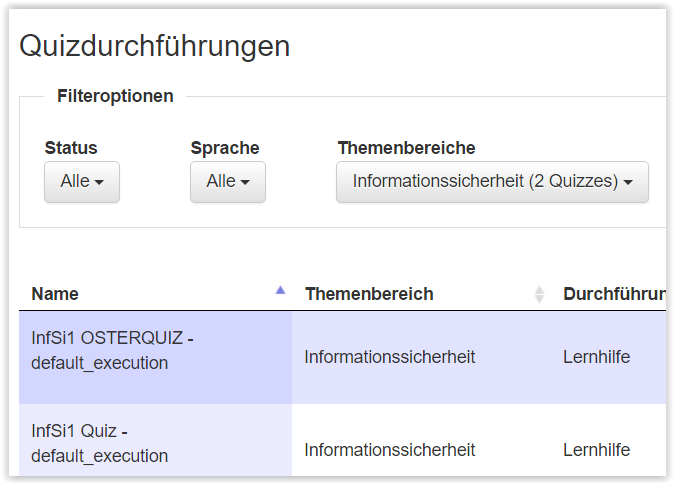
\includegraphics[width=0.45\textwidth]{Images/Neue_Filter_Mobile_Quiz.PNG}
	\caption{Filter der bestehenden (links) und der neuen (rechts) Mobile Quiz - Version}
	\cite{mobilequiz.ch}
\end{figure}



\newpage
\section{Schlussprodukt}

\begin{figure}[H]
	\centering
	\begin{itemize}
		\item Verbesserung der bestehenden Lösung
		\begin{itemize}
			\item \gls{Refactoring} und Fehlerbehebung
			\item Frage-Template
			\item Ablauf Quiz-Erstellung
			\item Design Quiz- und Frage-Erstellung
			\item Umgestaltung Startseite Teilnehmer/Ersteller
		\end{itemize}
		\item Neuerungen
		\begin{itemize}
			\item Fragen mit Bildern
			\item Feedback an Quiz-Ersteller
			\item Interessensgruppen und Filterumstellung
		\end{itemize}
	\end{itemize}
	\caption{Übersicht der Änderungen}
\end{figure}

Fasst man die Änderungen am bestehenden Mobile Quiz zusammen, so gab es einen überwiegenden Teil Überarbeitung der bestehenden Lösung sowie einen kleineren Teil von zusätzlichen Funktionalitäten. Die Verbesserungen kamen dabei zu einem Grossteil aus den Erkenntnissen der ersten \gls{Usability-Test}s, welche zu Beginn der Arbeit durchgeführt wurden. Diese sind im Anhang auf Seite \hyperlink{page.\getpagerefnumber{pdf:UTAW1}}{\getpagerefnumber{pdf:UTAW1}} zu finden. Die Wirkung davon blieb nicht aus, denn in der zweiten Durchführung gab es viel weniger Probleme mit dem Lösen der gegebenen Aufgaben, wie auf Seite \hyperlink{page.\getpagerefnumber{pdf:UTAW2}}{\getpagerefnumber{pdf:UTAW2}} ersichtlich ist.
Ausserdem haben die Fehlerbehebungen zu Beginn die Zuverlässigkeit von Mobile Quiz erhöht, was allen Benutzern zugute kommt und was das Vertrauen der Benutzer steigert.

Die Neuerungen ergänzen die Online Quiz-Plattform in verschiedenen Bereichen. Die Bild-Fragen geben dem Ersteller neue Möglichkeiten zur Wissensabholung und machen die Teilnahme an einem Quiz für Teilnehmer spannender.
Das Feedback an den Quiz-Ersteller erhöht die Kommunikation zwischen Teilnehmer und Quiz-Ersteller und soll dabei helfen Unklarheiten möglichst schnell aus dem Weg zu schaffen.
Schliesslich ist das Ziel der Interessensgruppen, dass Teilnehmer möglichst nur das sehen, was sie auch interessiert. Dadurch soll ein langes Suchen nach der gewünschten Quiz-Durchführung vermieden werden, wodurch die Bedienung als angenehm empfunden werden soll.

\bigskip

Alles in allem konnte Mobile Quiz durch die Umsetzung der oben beschriebenen Punkte zu einer verlässlicheren und bedienungsfreundlicheren Quiz-Plattform umgestaltet werden.

